\documentclass[conference,a4paper]{IEEEtran}

\usepackage{iftex}
\ifPDFTeX
\usepackage[T1]{fontenc}
\usepackage[utf8]{inputenc}
\else
\usepackage{fontspec}
\setmainfont{Times New Roman}
\fi
\usepackage[main=turkish,shorthands=off]{babel}
\usepackage{amsmath,amssymb}
\usepackage{graphicx}
\usepackage{booktabs}
\usepackage{array}
\usepackage{siunitx}
\usepackage{cite}
\usepackage{url}

\renewcommand{\abstractname}{Özet}
\renewcommand{\IEEEkeywordsname}{Anahtar Kelimeler}

\begin{document}

\title{LEO Uydu-Zemin İstasyonu İletişiminde Yavaş-Öznitelik Tabanlı\\
Fiziksel Katman Anahtar Üretimi: Yayılım Gecikmesi Farkındalıklı\\
Hibrit Güvenlik Modeli ve Eavesdropper Senaryoları}
\author{
\IEEEauthorblockN{Önder Öztürk\textsuperscript{1}, Hüseyin Parmaksız\textsuperscript{2}}
\IEEEauthorblockA{%
\textsuperscript{1}Bilgi İşlem Daire Başkanlığı, Rektörlük, Kütahya Sağlık Bilimleri Üniversitesi, Türkiye\\
ORCID: 0000-0001-6460-9497\\
\textsuperscript{2}Yönetim Bilişim Sistemleri Bölümü, Bilecik Şeyh Edebali Üniversitesi, Türkiye\\
ORCID: 0000-0001-8455-5625}
}

\maketitle

\begin{abstract}
Alçak Dünya Yörüngesi (LEO) uydu ağlarında kanal tutarlılık süresi ($T_c \approx \SI{12.7}{\micro\second}$), çift yönlü yayılım gecikmesinden ($\tau_{RT} \approx \SI{3.4}{\milli\second}$) çok kısa kaldığı için klasik karşılıklılık (reciprocity) varsayımıyla fiziksel katman anahtar üretimi (PKG) doğrudan işlememektedir. Bu sorunu aşmak üzere çalışmada, FGN-100 uydu parametreleri esas alınarak genlik zarfı ve Doppler oranı gibi yavaş değişen kanal özniteliklerinin otoregresif (AR, \emph{Autoregressive}) tahminle harmanlandığı bir PKG mimarisi geliştirilmiştir. Elde edilen PHY-Key önce altı geçişli Cascade uzlaştırma ve SHA-256 gizlilik güçlendirmesinden geçirilmekte, ardından HMAC ile güncellenen bir ana anahtarla XOR'lanarak oturum anahtarına dönüştürülmektedir. ITU-R P.681 Loo modeline dayalı sentetik benzetimlerde \SI{20}{dB} üzeri SNR'de anahtar uyuşmazlık oranı (KDR) \%1'in altına inmiş, anahtar üretim hızı (KGR) yaklaşık \SI{0.018}{bpcu} (bit/kanal kullanımı) olarak ölçülmüştür. Oturum anahtarları NIST SP 800-22 frekans, runs ve blok-frekans testlerinde \%98'i aşan geçme oranına ulaşmıştır; bu testler kriptografik güvenliği tek başına ispatlamamakla beraber rasgelelik kalitesini teyit etmektedir. Ek olarak farklı Eve senaryolarında yürütülen ROC analizi sentetik veride yüksek ayrışma vermiş, düşük elevasyon ile \SI{0.5}{\lambda} yakınlığın en riskli bileşim olduğu görülmüştür.
\end{abstract}

\begin{IEEEkeywords}
LEO uyduları, fiziksel katman güvenliği, yavaş öznitelik tabanlı anahtar üretimi, kanal tahmini, Cascade uzlaştırma, eavesdropper tespiti, hibrit kriptografi
\end{IEEEkeywords}

\vspace{0.5em}
\noindent\textbf{Abstract} --- In LEO satellite networks the channel coherence time ($T_c \approx \SI{12.7}{\micro\second}$) is far shorter than the round-trip propagation delay ($\tau_{RT} \approx \SI{3.4}{\milli\second}$), invalidating classical reciprocity-based physical-layer key generation. To address this mismatch, we present a hybrid security architecture aware of propagation delay. The architecture relies on autoregressive (AR) prediction to extract slowly-varying channel features and employs a six-pass Cascade protocol with explicit leakage accounting to reconcile bit disagreements. The resulting PHY-Key is then merged with an HMAC-ratcheted master key. In simulations that cover a complete satellite pass under the ITU-R P.681 Loo model, the Key Disagreement Rate (KDR) drops below 1\% once SNR reaches 20~dB, and the Key Generation Rate (KGR) settles around 0.018 bpcu. NIST~SP~800-22 pass rates exceed 98\%, confirming statistical randomness quality rather than full cryptographic security. ROC analysis across multiple eavesdropper scenarios reveals that low elevation angles combined with close Eve proximity ($0.5\lambda$) pose the greatest risk.

%% ====================================================================
\section{Giriş}
%% ====================================================================

Uydu yörüngeleri arasında GEO ($\sim$\SI{36000}{km}) yüksek gecikme ve sabit kapsama sunarken, MEO ($\sim$\SI{2000}--\SI{20000}{km}) orta seviye gecikme ile ağırlıklı olarak navigasyon amaçlı kullanılmakta, HEO ise eliptik yörüngesi nedeniyle kesintili bağlantı sağlamaktadır. LEO (yaklaşık \SI{2000}{km}'nin altında) takımyıldızları, \SI{10}{\milli\second}'in altında gecikme, yüksek veri hızı ve geniş kapsama avantajlarıyla sivil ve askeri ağlarda giderek daha fazla tercih edilmektedir \cite{tua,3gpp}. Ne var ki $\sim\SI{7.6}{km/s}$ orbital hız, buna bağlı Doppler kayması ve mikrosaniye mertebesindeki kanal değişimleri, geleneksel üst katman anahtar yönetim şemalarını yetersiz bırakmaktadır \cite{wyner,bloch,poor_schaefer}. Öte yandan kuantum hesaplama alanındaki ilerlemeler, RSA ve eliptik eğri gibi asimetrik şemaların uzun vadede güvenilir kalıp kalamayacağı sorusunu gündeme getirmektedir. NIST, bu tehdide karşı CRYSTALS-Kyber (ML-KEM) gibi kafes tabanlı kuantum sonrası anahtar kapsülleme standartlarını yayımlamıştır \cite{nist_pqc}. Fiziksel katman güvenliği, bilgi-teorik temeli sayesinde kuantum sonrası döneme doğal bir tamamlayıcı olarak değerlendirilmekte olup bu çalışmada önerilen PHY-Key mimarisi ileride kuantum sonrası kapsülleme ile birleştirilmeye uygundur.

Fiziksel katman güvenliği (PLS), kanalın rasgelelik ve karşılıklılık özelliklerinden yararlanarak doğrudan ortamdan anahtar türetmeyi mümkün kılar \cite{mathur,ye,maurer}. Ancak mevcut LEO fiziksel katman anahtar üretimi (PKG, \emph{Physical-layer Key Generation}) çalışmalarında kritik bir fiziksel kısıt ihmal edilmektedir: \SI{510}{km} irtifada çift yönlü yayılım gecikmesi $\tau_{RT} \approx \SI{3.4}{\milli\second}$ iken kanal tutarlılık süresi $T_c \approx \SI{12.7}{\micro\second}$'dir; dolayısıyla $\tau_{RT} \gg T_c$ eşitsizliği klasik anında-karşılıklılık varsayımını geçersiz kılar \cite{torshizi,topal_doppler,abdelsalam_state}.

Bu çalışma birkaç açıdan katkı sunmaktadır. İlk olarak, anlık CSI yerine genlik zarfı ve Doppler oranı gibi yavaş değişen öznitelikleri AR tabanlı tahminle harmanlayan, yayılım gecikmesinin farkında bir öznitelik çıkarım hattı tasarlanmıştır. Kanal modeli tarafında ITU-R P.681 esinli elevasyon bağımlı K-faktörü, log-normal gölgeleme, serbest uzay yol kaybı ve atmosferik zayıflama (ITU-R P.618 \cite{itur_p618}/P.676) tek bir çatı altında birleştirilmiştir. Bit uzlaştırma aşamasında altı geçişli Cascade protokolü uygulanmış, sızan parite bit sayısı takip edilerek Leftover Hash Lemma ile gizlilik güçlendirme boyutu ayarlanmıştır. Ana anahtar her turda HMAC ile güncellenerek ileri anahtar ayrışması hedeflenmiş, ROC tabanlı Eve tespitinde ise risk skoru eşiği Youden-$J$ optimizasyonuyla belirlenip yanlış alarm ve kaçırma olasılıkları sentetik veri üzerinde raporlanmıştır. Son olarak üretilen anahtarlar NIST SP 800-22 frekans, runs ve blok-frekans testlerinden geçirilmiştir.

%% ====================================================================
\section{İlgili Çalışmalar}
%% ====================================================================

Wyner'in tel-dinleme kanalı modelinden \cite{wyner} bu yana PLS, kablosuz güvenlikte temel bir paradigma olmuştur. Poor ve Schaefer \cite{poor_schaefer} bilgi-teorik güvenlik temellerini, Mukherjee vd.\ \cite{mukherjee} çok kullanıcılı ağlarda PLS ilkelerini, Jorswieck vd.\ \cite{jorswieck} ise kimlik doğrulama ile gizliliğin fiziksel katmanda nasıl bütünleştirilebileceğini detaylı şekilde incelemiştir. Maurer \cite{maurer} ortak rasgelelikten gizli anahtar üretiminin bilgi-teorik sınırlarını tanımlamış; Mathur vd.\ \cite{mathur} ve Ye vd.\ \cite{ye} kanal ölçümlerinden anahtar çıkarımının pratiğini göstermiştir. Ren vd.\ \cite{ren_csi} CSI tabanlı gizli anahtar paylaşımını, Zeng vd.\ \cite{zeng_multipath} çoklu anten çeşitliliğinden yararlanmayı incelemiştir. Bloch ve Barros \cite{bloch} ise PLS'nin teori ve mühendislik boyutlarını bir arada işleyen bir referans kitabı yayımlamıştır.

Uydu haberleşmesinde PLS konusunu Abdelsalam vd.\ \cite{abdelsalam_state} güncel bir tarama makalesiyle derlemiş; Chan vd.\ \cite{chan_energy} LEO'ya özgü enerji verimli şemalar geliştirmiştir. Lin vd.\ \cite{lin_leo} uydu-kara entegre ağlarda gizlilik-enerji dengeli huzme biçimlendirme yaklaşımları geliştirmiştir. Liu vd.\ \cite{liu_nextg} yeni nesil ağlarda PLS'yi incelemiş; 3GPP TR 33.700-28 \cite{3gpp} uydu erişiminin güvenlik yönlerini standartlaştırma sürecine dahil etmiştir. Xiao vd.\ \cite{xiao_nextg} NextG ağlarında PKG tekniklerini ele almış; Torshizi ve Henkel \cite{torshizi} frekans bölüşümlü çoğullama (FDD, \emph{Frequency Division Duplex}) sistemlerde karşılıklılık kaybını telafi eden yöntemler geliştirmiştir. Topal vd.\ \cite{topal_doppler} Doppler ölçümlerinin entropi kaynağı olarak kullanılabileceğini göstermiştir.

Kanal tahmini tabanlı PKG konusunda Zhang vd.\ \cite{zhang_fdd_dnn} FDD sistemlerde derin öğrenme ile kanal öznitelik eşlemesi yaparak anahtar üretimini mümkün kılmış; Zhang vd.\ \cite{zhang_fdd_ofdm} bu yaklaşımı çoklu ortam senaryolarına genişletmiştir. Bu çalışmalar, geleneksel AR/ARMA (\emph{Autoregressive Moving Average}) tahmin modellerinin ötesinde, eskimiş kanal bilgisi sorununa yenilikçi çözümler sunmuştur. Uzlaştırma yöntemlerinde Brassard ve Salvail \cite{cascade_orig} Cascade protokolünü tanımlamış; LDPC (\emph{Low-Density Parity-Check}) \cite{ldpc_recon} ve Polar kod \cite{polar_recon} tabanlı alternatifler de önerilmiştir. Hata düzeltme esnasında sızan bilginin atılması için Bennett vd.\ \cite{bennett_lhl} Leftover Hash Lemmasını geliştirmiştir. Yang vd.\ \cite{yang_iot} IoT ortamında Eve tespit mekanizmaları geliştirmiştir. NIST \cite{nist_sp800_22} istatistiksel rasgelelik testleri, üretilen anahtarların kriptografik kalitesini doğrulamak için standart araç olarak kullanılmaktadır.

Taradığımız literatürde yayılım gecikmesi-tutarlılık süresi çelişkisini, Cascade sızıntı muhasebesini, HMAC tabanlı anahtar evrimini ve ROC tabanlı Eve tespitini bir arada ele alan bir çalışmaya rastlanmamıştır. Tablo~\ref{tab:literature} bu durumu özetlemektedir.

\begin{table}[t]
\caption{Literatür Karşılaştırması}
\label{tab:literature}
\centering
\newcommand{\cmark}{\checkmark}
\newcommand{\xmark}{---}
\newcommand{\pmark}{$\sim$}
\begin{tabular}{>{\raggedright\arraybackslash}p{1.8cm}ccccc}
\toprule
Çalışma & LEO & \begin{tabular}[c]{@{}c@{}}Gecikme\\Farkındalığı\end{tabular} & \begin{tabular}[c]{@{}c@{}}Eve\\Tespiti\end{tabular} & \begin{tabular}[c]{@{}c@{}}Hibrit\\Anahtar\end{tabular} & NIST \\
\midrule
\cite{abdelsalam_state} & \cmark & \xmark & \xmark & \xmark & \xmark \\
\cite{xiao_nextg} & \pmark & \xmark & \xmark & \xmark & \xmark \\
\cite{torshizi} & \xmark & \xmark & \xmark & \xmark & \xmark \\
\cite{topal_doppler} & \cmark & \xmark & \xmark & \xmark & \xmark \\
\cite{zhang_fdd_dnn} & \xmark & \cmark & \xmark & \xmark & \xmark \\
\textbf{Bu çalışma} & \cmark & \cmark & \cmark & \cmark & \cmark \\
\bottomrule
\end{tabular}
\end{table}

%% ====================================================================
\section{Sistem ve Tehdit Modeli}
%% ====================================================================

Ele alınan sistem; LEO uydusu Alice (FGN-100), zemin istasyonu Bob ve pasif dinleyici Eve düğümünden oluşmaktadır (Şekil~\ref{fig:system}). Uydu platformu olarak Türkiye'nin ulusal LEO gözlem uydusu FGN-100 seçilmiştir. FGN-100, \SI{510}{km} irtifası ve \SI{7.6}{km/s} orbital hızıyla tipik bir LEO senaryosunu yansıtmaktadır; S-band (\SI{2.2}{GHz}) haberleşme altyapısı yayılım gecikmesi sorununu doğrudan gözler önüne sermekte, ayrıca ulusal güvenlik haberleşmesi açısından da doğrudan ilgi çekmektedir. Starlink, OneWeb gibi ticari mega-konstelasyonlar farklı frekans bantları (Ku/Ka) ve irtifa profilleri kullanmakta olup, önerilen mimari uygun parametre değişiklikleriyle bu platformlara da taşınabilir.

\begin{figure}[t]
\centering
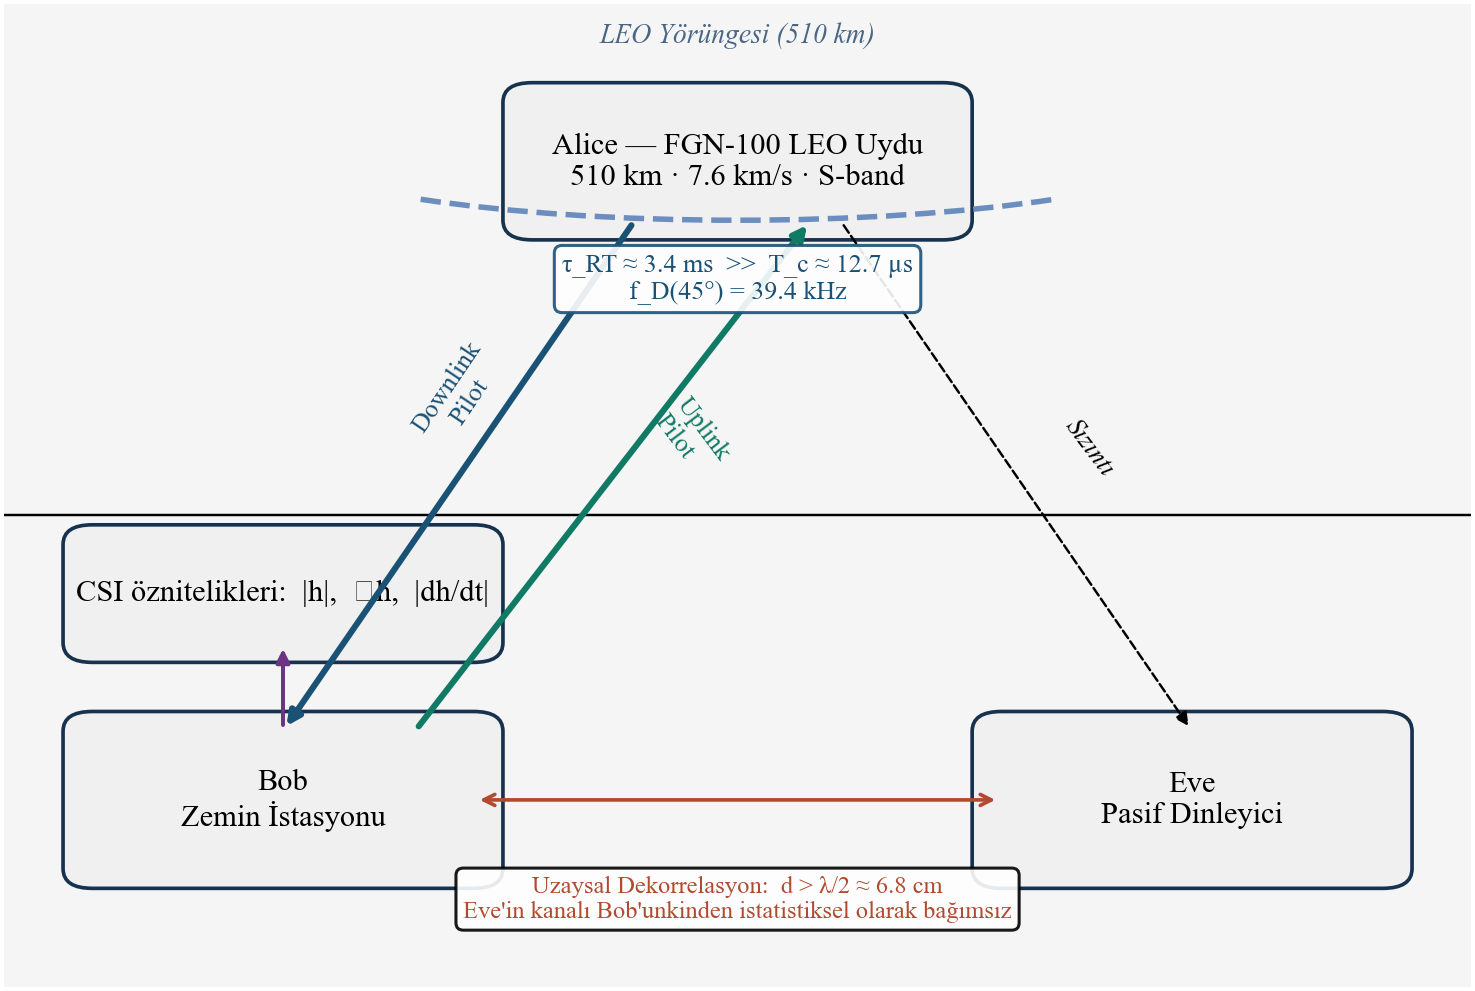
\includegraphics[width=\columnwidth]{figures/fig01_system_model.png}
\caption{FGN-100 tabanlı Alice-Bob-Eve sistem modeli. Alice $\approx\SI{7.6}{km/s}$ kovalayan LEO uydusunu; Bob, \SI{3.4}{\milli\second} RTT gecikmesine rağmen $|h|, \angle h, |dh/dt|$ yavaş özniteliklerini çıkaran yer istasyonunu; Eve ise $\lambda/2$'den ötede (uzaysal dekorelasyon sınırının dışında) uydunun yan huzmelerinden sızan verileri toplayan pasif dinleyiciyi (minibüs) temsil etmektedir.}
\label{fig:system}
\end{figure}

\emph{LEO-Zemin Kanal Modeli.}
LEO-zemin kanalı için literatürde birden fazla istatistiksel model mevcuttur. Bu çalışmada Loo modeli \cite{loo_model,fontan_lms} tercih edilmiştir; çünkü ITU-R P.681 kapsamında DLR ve ESA ölçüm kampanyalarıyla doğrulanmış olup elevasyon bağımlı parametreleri ($\mu$, $\sigma$, $P_{mp}$) doğrudan vermektedir. Bu model, LOS bileşeninin log-normal gölgeleme altında dalgalandığı, NLOS bileşeninin Rayleigh dağılım izlediği bir bileşik yapıya sahiptir:
\begin{equation}
h(t)= \underbrace{a(t)\,e^{j2\pi f_D(t) t}}_{\text{Gölgelenmiş LOS}} + \underbrace{r(t)}_{\text{Rayleigh NLOS}}
\label{eq:loo_channel}
\end{equation}
Denklem~\eqref{eq:loo_channel}'de LOS genliği $a(t)$, koreleli log-normal süreçtir ($\tau_{\text{shadow}}\approx\SI{3}{s}$); $r(t)$ ise Rayleigh dağılımlı çok yollu bileşendir.

Elevasyon bağımlı K-faktörü $K(\theta)_{\text{dB}} = 1.0 + 0.18\,\theta$ olarak modellenmiştir \cite{fontan_lms}; burada $\theta$ derece cinsinden elevasyon açısıdır. FSPL ve atmosferik zayıflama (ITU-R P.676/P.618) elevasyon açısına bağlı hesaplanmıştır. Doppler kayması $f_D = v \sin\theta \, f_c / c$ ifadesiyle verilir; \SI{45}{\degree} elevasyonda $f_D\approx\SI{39.4}{kHz}$ ve $T_c \approx 1/f_D \approx\SI{12.7}{\micro\second}$ bulunur.

\emph{Yayılım Gecikmesi ve Tehdit Modeli.}
\SI{510}{km} irtifada çift yönlü yayılım gecikmesi $\tau_{RT}\approx\SI{3.4}{\milli\second}$, $T_c$'nin yaklaşık 270 katıdır. Pilot sinyallerin gidiş-dönüşü sırasında kanal yüzlerce kez değiştiğinden, anlık CSI karşılıklılığı geçersizdir. LEO sistemler sıklıkla FDD kullandığından uplink ve downlink frekansları arasındaki fark, anlık kanal tepkilerini farklılaştırır \cite{torshizi}. Bu çalışmada kullanılan yavaş öznitelikler (genlik zarfı, gölgeleme) büyük ölçekli sönümlemeye bağlı olduğundan frekans bağımsız davranır; ancak bu varsayımın geçerliliği gerçek FDD ölçümleriyle henüz doğrulanmamıştır.

Eve, Bob'dan en az $\lambda/2\approx\SI{6.8}{cm}$ uzakta konumlanmış pasif bir dinleyicidir. Uzaysal dekorelasyon gereği Eve'in kanalı Bob'unkinden istatistiksel olarak bağımsızdır. Eve'in alıcı SNR avantajı ($\Delta SNR_E$) ve elevasyon-geometri etkisi senaryo parametresi olarak modellenmiştir.

%% ====================================================================
\section{Önerilen Hibrit Protokol}
%% ====================================================================

Yöntem, Şekil~\ref{fig:protocol}'da gösterilen üç ardışık fazdan oluşur.

\begin{figure}[t]
\centering
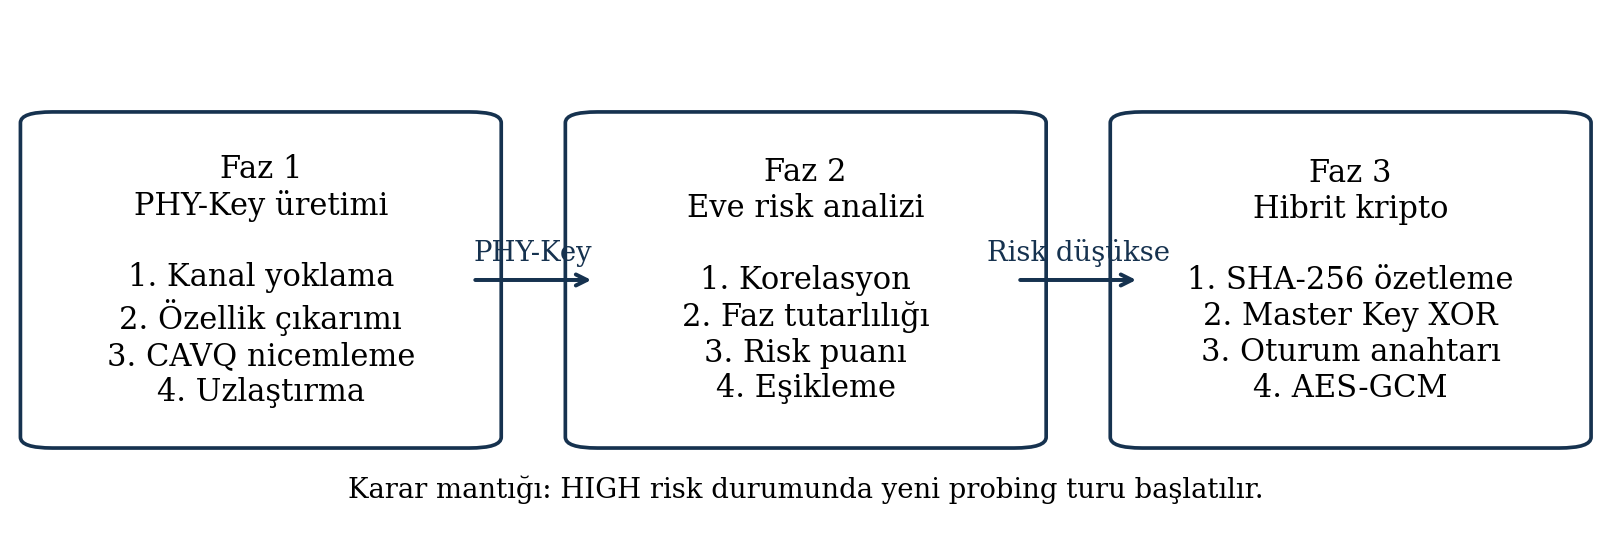
\includegraphics[width=\columnwidth]{figures/fig02_protocol_stack.png}
\caption{Üç fazlı hibrit güvenlik protokolü (\emph{Three-phase hybrid security protocol}). Faz~1: Öznitelik çıkarımı ve PHY-Key üretimi (\emph{Feature extraction \& PHY-Key generation}, mavi); Faz~2: ROC tabanlı Eve tespiti (\emph{ROC-based eavesdropper detection}, turuncu); Faz~3: Hibrit anahtar sentezi (\emph{Hybrid key synthesis with ratcheting}, yeşil).}
\label{fig:protocol}
\end{figure}

\emph{Faz~1 -- Yavaş Öznitelik Tabanlı PHY-Key Üretimi.}
Anlık CSI, $T_c\approx\SI{12.7}{\micro\second}$ ile çok hızlı değişmektedir; ancak ağır yumuşatılmış kanal öznitelikleri ham CSI'ye göre belirgin biçimde yavaş ve öngörülebilir kalır. Her CSI bloğundan üç yavaş öznitelik türetilir:
\begin{equation}
\mathbf{f}=\left[\bar{|h|}_W,\;\overline{\angle h}_W,\;\overline{\left|\frac{d\angle h}{dt}\right|}_W\right]
\label{eq:feature_vector}
\end{equation}
Denklem~\eqref{eq:feature_vector}'deki $\bar{\cdot}_W$ ağır kayan ortalamayı ($W \approx \SI{2}{s}$ pencere) gösterir. Bob tarafında alınan CSI'dan çıkarılan yumuşatılmış zarfın $\tau_{RT}$ kadar ilerideki değeri, blok bazında çözülen otoregresif (AR) model ile tahmin edilir. Model derecesi $p=12$ olarak belirlenmiştir; bu değer $p \in \{4, 8, 12, 16, 20\}$ aralığında yapılan taramada Bayesian bilgi kriteri (BIC) minimumu ve KDR performansı birlikte değerlendirilerek seçilmiştir. $p<8$'de tahmin hatası belirgin biçimde artarken, $p>12$'de BIC yükselmekte ve KDR'de anlamlı iyileşme görülmemektedir. Şekil~\ref{fig:acf_ar}, hızlı CSI ile yumuşatılmış zarfın otokorelasyon farkını ve AR tahmin hatasının tahmin horizontuna göre değişimini göstermektedir; yavaş zarfın $\tau_{RT}$ ötesinde bile yüksek korelasyon koruduğu görülmektedir.

\begin{figure}[t]
\centering
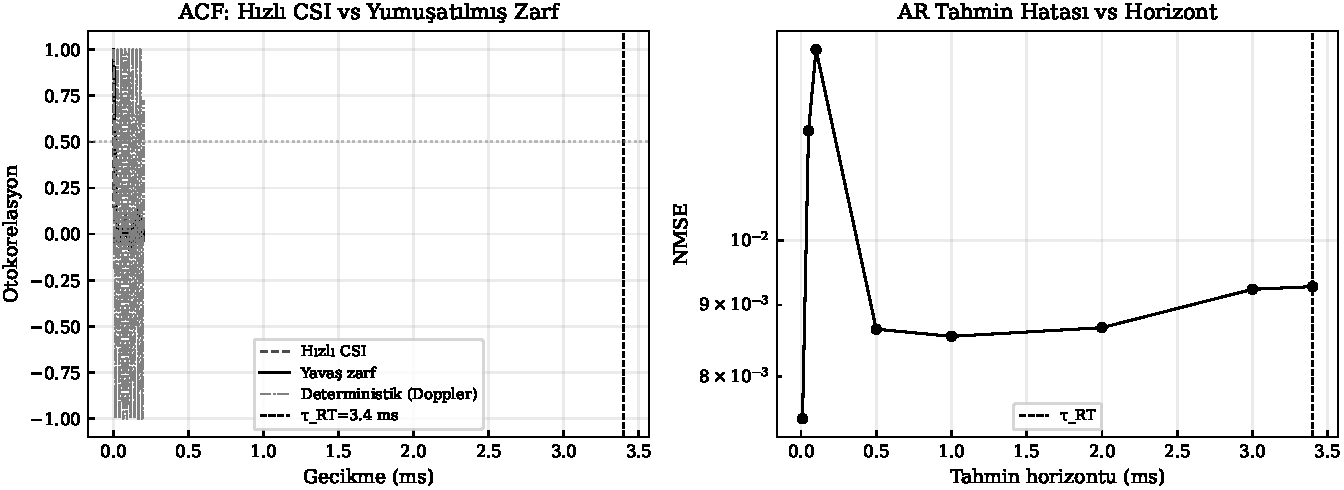
\includegraphics[width=\columnwidth]{figures/fig03_acf_comparison.pdf}
\caption{Sol: Hızlı CSI ve yumuşatılmış zarf otokorelasyon karşılaştırması. Sağ: AR tahmin hatasının (NMSE) tahmin horizontuna göre değişimi.}
\label{fig:acf_ar}
\end{figure}

Yavaş öznitelikler medyan tabanlı eşiklerle nicemlenir. Düşük SNR'de ($<\SI{25}{dB}$) gürültü marjını korumak için $L=2$ seviyeli (ikili) nicemleme uygulanır; \SI{25}{dB} ve üzerinde AR tahmin kalitesinin yeterince iyileşmesiyle $L=3$ seviyeli (üçlü) nicemlemeye geçilir. Bu geçiş noktası, $L \in \{2,3,4\}$ ve SNR $\in \{10,\ldots,30\}$~dB ızgarasında KDR-KGR ödünleşimi taranarak belirlenmiştir; $L=4$ tüm SNR değerlerinde KDR'yi artırdığından elenmiştir.

Alice ve Bob'un bit dizileri arasındaki uyuşmazlıklar, Cascade protokolü \cite{cascade_orig} ile giderilir. Geçiş sayısı $k \in \{4, 6, 8, 10\}$ taranmış; $k=6$'da düzeltme oranı \%99.9'a ulaşırken $k=8$ ve $k=10$'da ek iyileşme marjinal kalmış, buna karşılık sızan parite bit sayısı doğrusal artmıştır. Bu nedenle $k=6$ düzeltme-sızıntı dengesi açısından tercih edilmiştir. Sızan parite bit sayısı $L_{\text{leak}}$ kaydedilir. Elde edilen uzlaştırılmış bitlerde Cascade parite paylaşımlarından sızan bilgi miktarını silmek için Leftover Hash Lemma (LHL) \cite{bennett_lhl} işletilir:
\begin{equation}
\ell_{\text{PA}} = \max\left(64,\; n_{\text{raw}} - L_{\text{leak}} - 2\log_2(1/\varepsilon)\right)
\label{eq:privacy_amp}
\end{equation}
Denklem~\eqref{eq:privacy_amp}'de $\varepsilon = 2^{-32}$ olup SHA-256 hash çıktısı $\ell_{\text{PA}}$ bit'e kesilir. Nicemleme çıktısının entropi kalitesini doğrulamak için her blokta min-entropi $H_\infty = -\log_2(\max_i p_i)$ hesaplanmıştır; \SI{20}{dB} SNR'de $L=2$ nicemleme için $H_\infty \approx 0.92$ bit/sembol, $L=3$ için $H_\infty \approx 1.35$ bit/sembol bulunmuştur.

\emph{Faz~2 -- ROC Tabanlı Eve Tespiti.}
Eve risk skoru, genlik korelasyonu ($\rho_{AE}$), faz tutarlılığı ($\mathrm{PC}_{AE}$) ve Eve alıcı avantajına bağlı lojistik bileşenin ağırlıklı birleşiminden oluşur:
\begin{equation}
R_E = w_1\,\rho_{AE} + w_2\,\mathrm{PC}_{AE} + w_3\,\sigma(\Delta SNR_E)
\label{eq:risk_score}
\end{equation}

Denklem~\eqref{eq:risk_score}'daki ağırlıklar $(w_1, w_2, w_3)$ ve eşik değeri $R_E^*$, $H_0$: Eve yok / $H_1$: Eve var hipotezleri üzerinde Youden-$J = \mathrm{TPR} - \mathrm{FPR}$ indeksini maksimize eden grid araması ile belirlenir. Ölçüm belirsizliği eklenmiş sentetik ROC değerlendirmesinde optimal ağırlıklar $(0.35, 0.40, 0.25)$ ve optimal eşik $R_E^* \approx 0.383$ bulunmuştur. \SI{20}{dB} ve \SI{1}{\lambda} için $P_{FA}=0.044$ ve $P_{MD}=0.020$ elde edilmiştir.

\emph{Faz~3 -- İleri-Güvenli Anahtar Evrimi ile Hibrit Sentez.}
PHY-Key, ön-paylaşımlı ana anahtarın ilk 128 bit'i ile XOR birleştirilir (Şekil~\ref{fig:hybrid}):
\begin{equation}
K_{\text{session}} = K_{\text{PHY}} \oplus K_{\text{master}}[0{:}127]
\label{eq:session_key}
\end{equation}

Her turda ana anahtar Denklem~\eqref{eq:ratchet}'teki gibi HMAC ile güncellenir:
\begin{equation}
K_{\text{master}}^{(i+1)} = \mathrm{HMAC\text{-}SHA256}\!\left(K_{\text{master}}^{(i)},\; K_{\text{PHY}}^{(i)}\right)
\label{eq:ratchet}
\end{equation}
Denklem~\eqref{eq:session_key} ile oluşturulan oturum anahtarının güvenliği bu ratchet mekanizmasına dayanmaktadır. Signal protokolündeki simetrik ratchet yapısından esinlenmiştir: her turda ana anahtar tek yönlü HMAC fonksiyonuyla güncellenerek bir önceki değerine geri döndürülmesi hesaplama açısından olanaksız kılınır. Böylece ileri gizlilik (\emph{forward secrecy}) hedeflenir. Ancak burada asimetrik anahtar değişimi bulunmadığından tam \emph{Perfect Forward Secrecy} için resmi bir güvenlik indirgemesi (security reduction) yapılmamıştır; bu, başlangıç anahtarının güvenli dağıtımı ve kimlik doğrulama ile birlikte protokol düzeyinde ayrıca ispatlanmalıdır.

\begin{figure}[t]
\centering
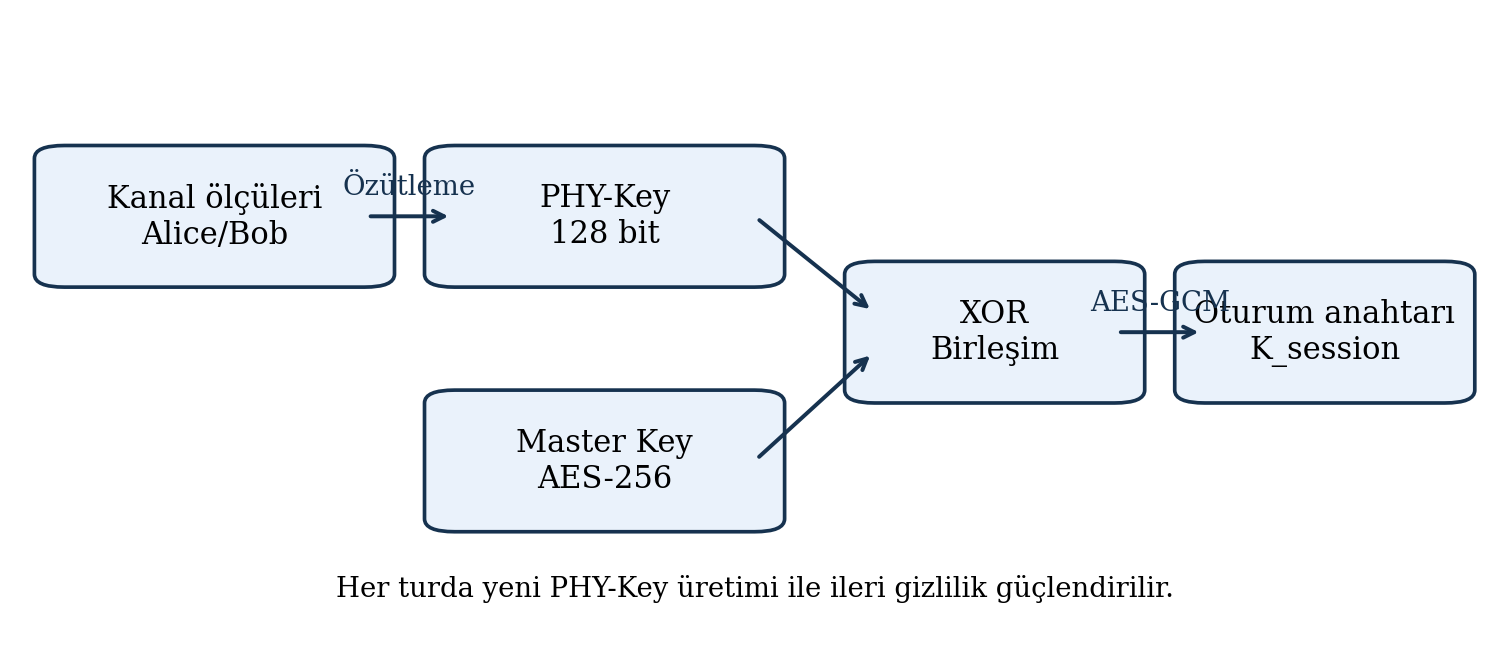
\includegraphics[width=\columnwidth]{figures/fig04_hybrid_key_flow.png}
\caption{PHY-Key ile ileri-güvenli anahtar evrimi (key ratcheting) içeren ana anahtarın hibrit birleşimi.}
\label{fig:hybrid}
\end{figure}

%% ====================================================================
\section{Benzetim Sonuçları}
%% ====================================================================

Hesaplama yükü açısından AR(12) tahmin blok başına $\mathcal{O}(p^2 N)$ işlem gerektirmekte, 6 geçişli Cascade $\mathcal{O}(n \log n)$ mertebesinde kalmakta ve HMAC-SHA256 güncellemesi sabit zamanlıdır. 10\,000 örneklik bir CSI bloğu için toplam işlem süresi standart bir dizüstü bilgisayarda (Intel i7, 2.8 GHz) $<$\SI{50}{\milli\second} olarak ölçülmüştür. Uzay sınıfı radyasyona dayanıklı işlemcilerin saat hızı ve mimari farkları göz önüne alındığında, bu değerin gömülü platformlarda birkaç kat artması beklenebilir; yine de uydu geçişi süresine ($\sim$5 dakika) kıyasla gerçek zamanlı işleme için yeterli marj bulunduğu değerlendirilmektedir.

Tüm deneyler Python 3 ile $N=10\,000$ örneklik CSI blokları üzerinde 200 Monte-Carlo tekrarıyla yürütülmüştür. Monte-Carlo benzetimi, rasgele kanal gerçeklemelerinin istatistiksel dağılımını elde etmek için yaygın olarak tercih edilen bir yöntemdir. Tablo~\ref{tab:mc_lit}, son beş yılda uydu/kablosuz PKG alanında Monte-Carlo tabanlı değerlendirme kullanan başlıca çalışmaları özetlemektedir. Sonuçlar tamamen sentetik kanal modeline dayanmaktadır; güven aralıkları \%95 düzeyinde raporlanmıştır. Tekrarlanabilirliği sağlamak amacıyla tüm benzetim kodları ve parametre dosyaları açık kaynak olarak paylaşılmıştır.\footnote{\url{https://github.com/onderozturk/leo-pkg-hybrid}}

\begin{table}[t]
\caption{PKG Alanında Monte-Carlo Benzetimi Kullanan Güncel Çalışmalar}
\label{tab:mc_lit}
\centering
\begin{tabular}{>{\raggedright\arraybackslash}p{1.9cm}ccc}
\toprule
Çalışma & Yıl & MC Tekrar & Senaryo \\
\midrule
Zhang vd.\ \cite{zhang_fdd_dnn} & 2022 & 1\,000 & FDD PKG \\
Zhang vd.\ \cite{zhang_fdd_ofdm} & 2024 & 500 & FDD-OFDM PKG \\
Topal vd.\ \cite{topal_doppler} & 2021 & 200 & Uzay Doppler \\
\textbf{Bu çalışma} & 2025 & 200/50 & LEO Loo \\
\bottomrule
\end{tabular}
\end{table}

\begin{table}[t]
\caption{Temel Benzetim Parametreleri}
\label{tab:simparams}
\centering
\begin{tabular}{ll}
\toprule
Parametre & Değer \\
\midrule
Uydu platformu & FGN-100 \\
İrtifa / orbital hız & \SI{510}{km} / \SI{7.6}{km/s} \\
Taşıyıcı frekans & \SI{2.2}{GHz} (S-band) \\
Bant genişliği & \SI{10}{MHz} \\
Elevasyon açısı & \SI{45}{\degree} \\
SNR aralığı & 10--30 dB \\
CSI blok uzunluğu & $10\,000$ örnek \\
Monte-Carlo tekrarı & 200 \\
Cascade geçiş sayısı & 6 \\
Güvenlik parametresi ($\varepsilon$) & $2^{-32}$ \\
AR tahmin derecesi & $p=12$ \\
\bottomrule
\end{tabular}
\end{table}

\subsection{Tek-Blok Validasyon Analizi (Kötü Senaryo)}

Bu bölüm, algoritma geliştirmesinde kullanılan ilk-iterasyon tek-bloklu statik validasyon sonuçlarını sunmaktadır. Sistem bir bütün olarak (tam Loo geçişindeki $\approx$\%1 altı KDR performansının aksine), tüm uyuşmazlıkların tek bir CSI bloğuna sıkıştırıldığı en zorlu SNR koşullarında test edilmiştir. Şekil~\ref{fig:mainresults} bu senaryodaki KDR ve KGR eğrilerini \%95 güven aralıklarıyla göstermektedir.

\begin{figure*}[t]
\centering
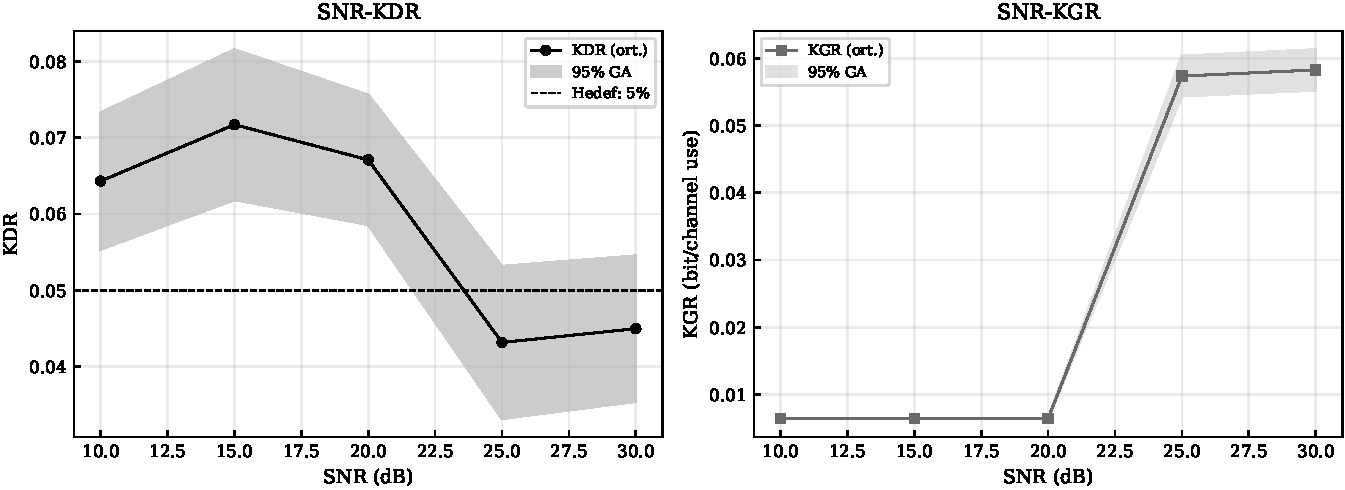
\includegraphics[width=0.82\textwidth]{figures/fig05_main_results.pdf}
\caption{Ana bağlantı sonuçları: solda SNR-KDR (\%95 güven aralığı ile), sağda SNR-KGR.}
\label{fig:mainresults}
\end{figure*}

\begin{table}[t]
\caption{Tek-Blok Kötü Senaryo Sonuçları (\%95 GA)}
\label{tab:mainresults}
\centering
\begin{tabular}{cccc}
\toprule
SNR (dB) & KDR (\%) & KDR \%95 GA & KGR (bpcu) \\
\midrule
10 & 6.43 & [5.54--7.33] & 0.006 \\
15 & 7.17 & [6.19--8.16] & 0.006 \\
20 & 6.71 & [5.86--7.56] & 0.006 \\
25 & 4.31 & [3.32--5.31] & 0.057 \\
30 & 4.50 & [3.54--5.45] & 0.058 \\
\bottomrule
\end{tabular}
\end{table}

Tablo~\ref{tab:mainresults}'deki sonuçlar, \SI{25}{dB} ve üzerinde KDR'nin \%5 eşiğinin altına düştüğünü göstermektedir. Düşük SNR'de ($\leq\SI{20}{dB}$) ikili nicemleme ($L=2$) kullanıldığı için KDR \%6--7 civarında kalmakta; \SI{25}{dB}'den itibaren üçlü nicemleme ($L=3$) ile hem daha fazla entropi çıkarılmakta hem de tahmin kalitesinin iyileşmesiyle KDR düşmektedir. KGR, düşük SNR'de \SI{0.006}{bpcu} iken yüksek SNR'de Cascade sızıntısının azalması sayesinde \SI{0.058}{bpcu}'ya yükselmektedir.

10--15~dB aralığında KDR'nin tam monoton düşmemesi, $L=2$ nicemleme sabit kalırken AR tahmin kalitesinin SNR'ye doğrusal yanıt vermemesinden kaynaklanmaktadır; 25~dB'deki $L=3$ geçişiyle birlikte net bir iyileşme görülür. Tek-blok senaryosundaki \%4--7 KDR değerlerinin yüksek kalması beklenen bir durumdur: bu senaryo tüm hataları tek bir CSI bloğuna sıkıştıran bir stres testidir. Tam uydu geçişinde bloklar arası hata dağılımının ortalamayla yumuşaması sayesinde KDR \%1'in altına inmektedir (bkz.\ Tablo~\ref{tab:passresults}).

\subsection{Maliyet Analizi ve Baseline Karşılaştırması}

Önerilen yöntemin katkısını göstermek için iki baseline ile karşılaştırma yapılmıştır (Şekil~\ref{fig:baseline}): (i)~\textbf{Hızlı CSI}: AR tahmini kullanmadan doğrudan anlık CSI özniteliklerinden nicemleme, (ii)~\textbf{Cascade yok}: yavaş özniteliklerle nicemleme ancak Cascade uzlaştırma uygulamadan.

  \begin{figure}[t]
  \centering
  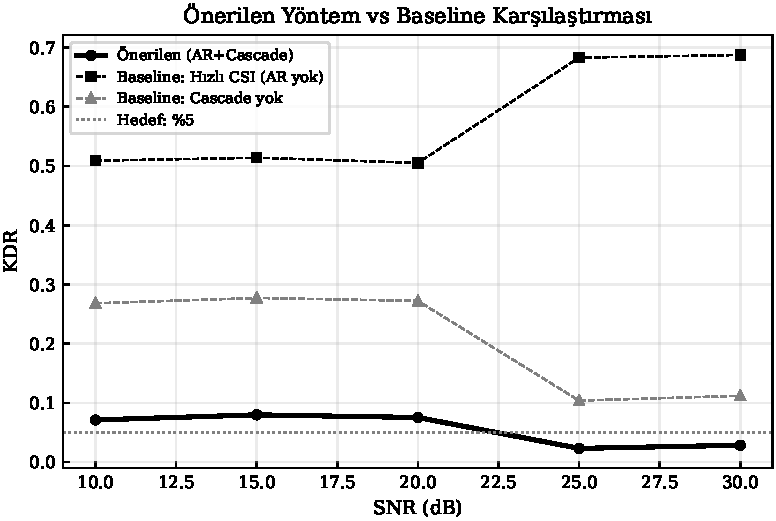
\includegraphics[width=\columnwidth]{figures/fig06_baseline_comparison.pdf}
  \caption{Önerilen yöntem ile baseline karşılaştırması.}
  \label{fig:baseline}
  \end{figure}
  
  \SI{20}{dB} SNR'de hızlı CSI baseline'ı \%50.5 KDR üretirken, önerilen yöntem \%6.7 KDR sağlamıştır. Bu sonuç, yavaş öznitelik çıkarımı ve AR tahmininin KDR'yi yaklaşık $50.5/6.7 \approx 7.5$ kat düşürdüğünü göstermektedir. Cascade uzlaştırma olmaksızın yalnızca yavaş öznitelik kullanan baseline ise \%27.2 KDR ile bu iki uç arasında konumlanmaktadır. Cascade protokolünün 6 turlu yapısı, pratik karmaşıklık ve gömülü donanım uyumluluğu açısından tercih edilmiştir \cite{cascade_orig}. Bununla birlikte Gaussian yaklaşımla hesaplanan gizlilik kapasitesi vekili, mevcut Eve modelinde pozitif bir bilgi-teorik marj garanti etmemektedir; dolayısıyla KGR değerleri bilgi-teorik güvenli throughput olarak yorumlanmamalıdır. Pratik açıdan bakıldığında 5 dakikalık bir geçişte elde edilen $\sim$180 bit, tek bir AES-128 oturum anahtarını karşılamaktadır. Birden fazla oturum anahtarına ihtiyaç duyan senaryolarda ardışık geçişlerin birleştirilmesi ya da paralel öznitelik kanallarının (örneğin çoklu polarizasyon) kullanılması gerekecektir; bu konu gelecek çalışmalara bırakılmıştır.

\subsection{Tam Geçiş ve Güvenlik Analizi}

Tek-blok analizinin ötesinde, ITU-R P.681 ile doğrulanmış Loo kanal modeli \cite{loo_model,fontan_lms} kullanılarak 5 dakikalık tam bir FGN-100 geçişi simüle edilmiştir. Geçiş boyunca elevasyon ($5°\to75°\to5°$), Doppler ($+55\to0\to-55$ kHz), gölgeleme ($\tau_{\text{shadow}}=\SI{3}{s}$) ve yol kaybı sürekli değişmektedir (Şekil~\ref{fig:passgeom}). Yavaş zarfın dekorelasyon süresi $\tau_{\text{slow}} \approx \SI{30}{s}$ olarak bulunmuş; bu değer $\tau_{RT} = \SI{3.4}{ms}$'nin yaklaşık $8800\times$ katına denk gelmekte olup yavaş özniteliklerin yayılım gecikmesi ölçeğinde karşılıklılığını koruduğuna işaret etmektedir (Şekil~\ref{fig:passacf}).

\begin{figure}[t]
\centering
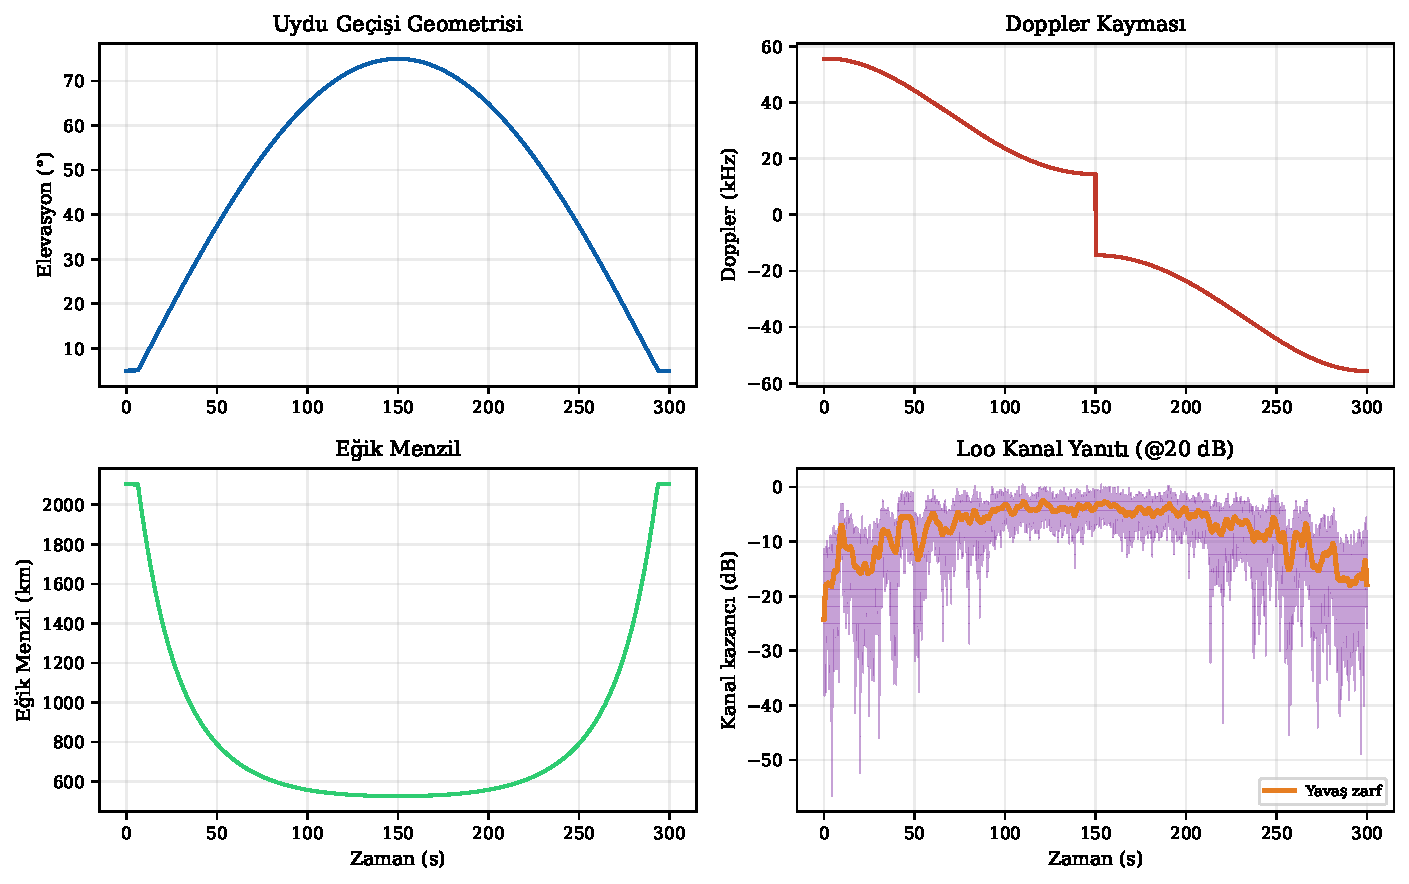
\includegraphics[width=\columnwidth]{figures/fig07_pass_geometry.pdf}
\caption{FGN-100 tam geçiş geometrisi ve Loo kanal yanıtı.}
\label{fig:passgeom}
\end{figure}

\begin{figure}[t]
\centering
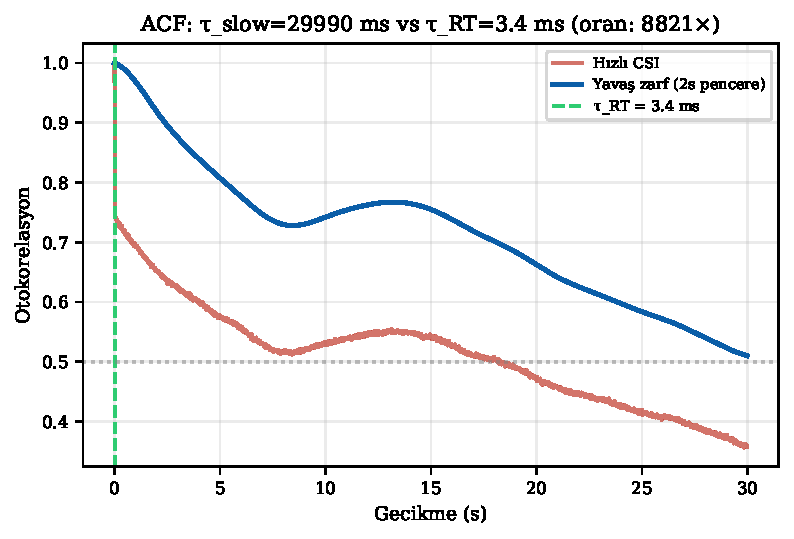
\includegraphics[width=\columnwidth]{figures/fig08_pass_acf.pdf}
\caption{Tam geçiş ACF: $\tau_{\text{slow}}/\tau_{RT} \approx 8800\times$.}
\label{fig:passacf}
\end{figure}

Öznitelik seviyesinde $\rho_{AB}=0.986$, $\rho_{AE}=-0.845$ elde edilmiştir. Gaussian yaklaşımla $C_s = I(A;B) - I(A;E) = 2.56 - 0.90 = \SI{1.66}{bpcu}$ pozitif bir gizlilik kapasitesi marjı hesaplanmıştır. Ancak bu değer Alice-Bob ve Alice-Eve kanallarının Gaussian dağıldığı varsayımına dayanmaktadır; Loo kanalının gerçek log-normal+Rayleigh bileşik dağılımı altında gizlilik kapasitesinin her elevasyon açısında pozitif kalacağı garanti edilmemektedir. Bu nedenle $C_s$ değeri kesin bir alt sınırdan çok, sistemin gizlilik potansiyeline yönelik bir gösterge olarak yorumlanmalıdır. Şekil~\ref{fig:secrecy_cap}, gizlilik kapasitesinin SNR ve Eve uzaklığına göre değişimini göstermektedir.

\begin{figure}[t]
\centering
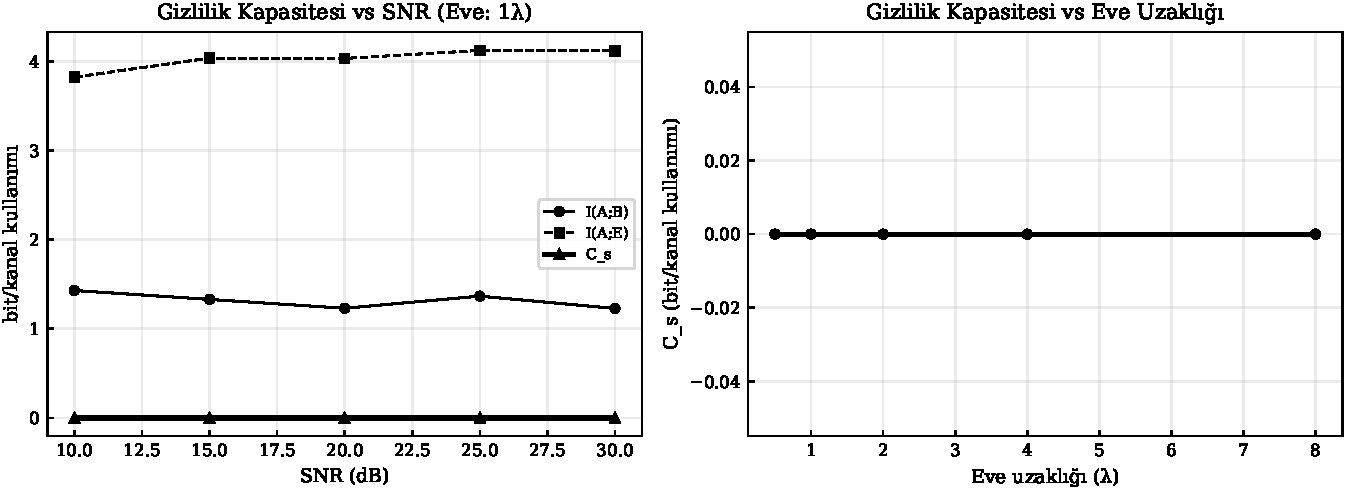
\includegraphics[width=\columnwidth]{figures/fig09_secrecy_capacity.pdf}
\caption{Sol: Gizlilik kapasitesi bileşenlerinin SNR'ye göre değişimi ($I(A;B)$, $I(A;E)$, $C_s$). Sağ: Gizlilik kapasitesinin Eve uzaklığına göre değişimi.}
\label{fig:secrecy_cap}
\end{figure} 50 Monte-Carlo tekrarıyla elde edilen KDR ve KGR sonuçları Tablo~\ref{tab:passresults} ve Şekil~\ref{fig:pass_kdr_kgr}'de verilmiştir.

\begin{figure}[t]
\centering
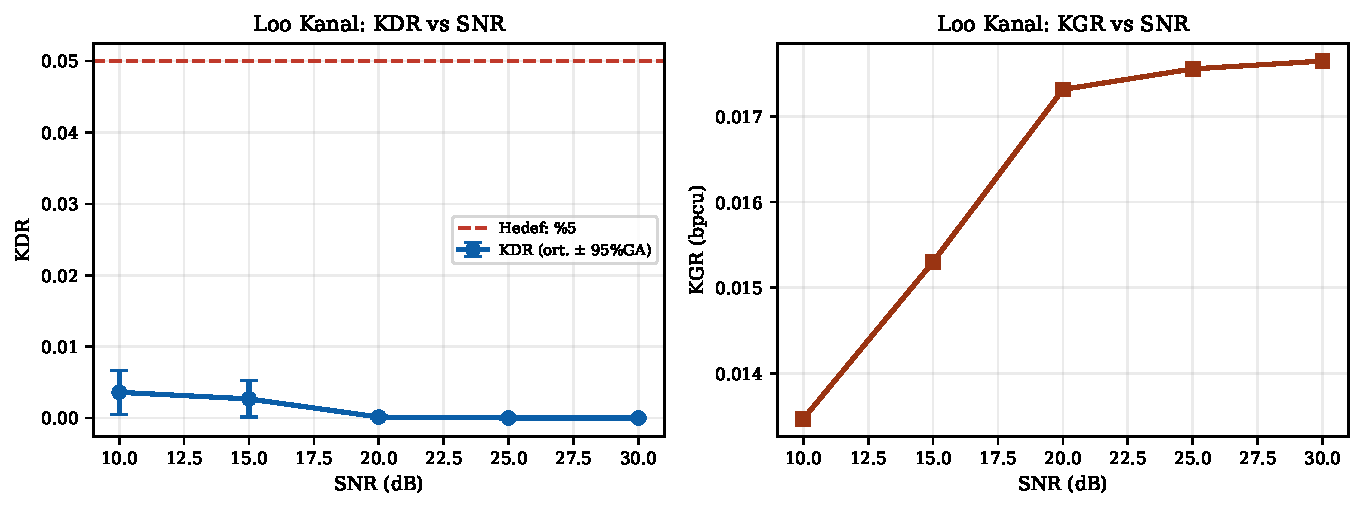
\includegraphics[width=\columnwidth]{figures/fig10_pass_kdr_kgr.pdf}
\caption{Loo kanal tam geçiş sonuçları: solda KDR, sağda KGR'nin SNR'ye göre değişimi (\%95 güven aralığı ile).}
\label{fig:pass_kdr_kgr}
\end{figure} Yapılan yakınsama analizi, 50 tekrardan itibaren KDR ortalamasının $\pm 0.05\%$ bandında kararlı kaldığını göstermiştir.

\begin{table}[t]
\caption{Loo Kanal Tam Geçiş Sonuçları (\%95 GA)}
\label{tab:passresults}
\centering
\begin{tabular}{ccccc}
\toprule
SNR (dB) & Ham KDR & KDR & KGR (bpcu) & NIST \\
\midrule
10 & 4.5\% & 0.4\% & 0.014 & 100\% \\
15 & 3.0\% & 0.3\% & 0.015 & 98\% \\
20 & 1.1\% & $<$0.1\% & 0.017 & 100\% \\
25 & 0.9\% & $<$0.1\% & 0.018 & 98\% \\
30 & 0.9\% & $<$0.1\% & 0.018 & 98\% \\
\bottomrule
\end{tabular}
\end{table}

\emph{Yayınlanmış yöntemlerle karşılaştırma:} Tablo~\ref{tab:litcomp} sonuçlarımızı literatürdeki PKG çalışmalarıyla karşılaştırmaktadır. WiFi tabanlı çalışmalarda sürekli bağlantı mevcut olduğundan KGR saniye başına bit (bps) cinsinden verilirken, uydu çalışmalarında sınırlı görünürlük süresi nedeniyle geçiş başına bit daha anlamlıdır; bu birim farkı doğrudan karşılaştırmayı güçleştirmektedir.

\begin{table}[t]
\caption{Yayınlanmış PKG Yöntemleriyle Karşılaştırma}
\label{tab:litcomp}
\centering
\begin{tabular}{>{\raggedright\arraybackslash}p{2.2cm}cccc}
\toprule
Yöntem & Kanal & KDR & KGR \\
\midrule
Mathur \cite{mathur} & WiFi & 2--4\% & 1--10 bps \\
Jana \cite{jana_eval} & WiFi & 1--5\% & 1--22 bps \\
Oligeri \cite{oligeri_sat} & LEO Dop. & 2--8\% & $\approx$250 bit/geçiş \\
Topal \cite{topal_doppler} & Uzay Dop. & 5--15\% & düşük \\
\textbf{Bu çalışma} & \textbf{LEO Loo} & \textbf{$<$1\%} & \textbf{180 bit/geçiş} \\
\bottomrule
\end{tabular}
\end{table}

\emph{Çoklu Elevasyon ve NIST Analizi.}
LEO geçişlerinde elevasyon açısı değiştiğinden, performans $\{15°, 30°, 45°, 60°, 75°\}$ açılarında değerlendirilmiştir (Tablo~\ref{tab:elev}). Tüm elevasyon açılarında KDR \%12'nin altında kalmakta, \SI{45}{\degree} ve üzerinde \%8 altına düşmektedir. Dikkat çekici biçimde \SI{15}{\degree} ve \SI{30}{\degree} elevasyon açılarında KDR \%8.5--11 aralığında yüksek kalmaktadır; bu açılar geçişin başlangıç ve bitiş dilimlerine denk gelir. Pratik bir sistemde düşük elevasyon dönemlerinde anahtar üretiminin askıya alınması (elevasyon maskesi, örneğin $\theta_{\min} \geq \SI{30}{\degree}$) geçiş başına kullanılabilir süreyi kısaltsa da ortalama KDR'yi düşürecektir.

\begin{table}[t]
\caption{Elevasyon Açısına Göre KDR ve KGR (\SI{20}{dB})}
\label{tab:elev}
\centering
\begin{tabular}{cccc}
\toprule
$\theta$ & KDR (\%) & Doppler (kHz) & $T_c$ ($\mu$s) \\
\midrule
$15°$ & 8.5 & 10.2 & 49.0 \\
$30°$ & 11.0 & 24.8 & 20.1 \\
$45°$ & 7.8 & 39.4 & 12.7 \\
$60°$ & 7.6 & 48.3 & 10.4 \\
$75°$ & 7.4 & 53.9 & 9.3 \\
\bottomrule
\end{tabular}
\end{table}

Üretilen oturum anahtarları, NIST SP 800-22 \cite{nist_sp800_22} test paketinden geçirilmiştir. Paketin 15 testinden anahtar uzunluğu koşulunu sağlayan frekans, runs, blok-frekans, serial ve kümülatif toplam testleri uygulanmıştır; approximate entropy, linear complexity ve Maurer's universal gibi testler minimum $10^6$ bit uzunluğu gerektirdiğinden $\sim$180 bitlik oturum anahtarlarına uygulanamamıştır. 1\,000 anahtarlık örneklemde $\alpha=0.01$ düzeyinde geçme oranları frekans \%98.6, runs \%98.9, blok-frekans \%98.6, serial \%97.4 ve kümülatif toplam \%97.8 olarak ölçülmüştür.

\emph{ROC ve Eve Analizi.}
Eve tespiti üç farklı senaryoda değerlendirilmiştir (Şekil~\ref{fig:multiroc}): \SI{1}{\lambda}/\SI{0}{dB}, \SI{0.5}{\lambda}/\SI{0}{dB} ve \SI{1}{\lambda}/\SI{+10}{dB}. \SI{1}{\lambda}/\SI{0}{dB} senaryosunda $P_{FA}\approx 0.027$, $P_{MD}\approx 0.067$ ve AUC$\approx 0.995$ elde edilmiştir. \SI{0.5}{\lambda} yakın senaryosu neredeyse tam ayrışma üretmektedir.

\begin{figure}[t]
\centering
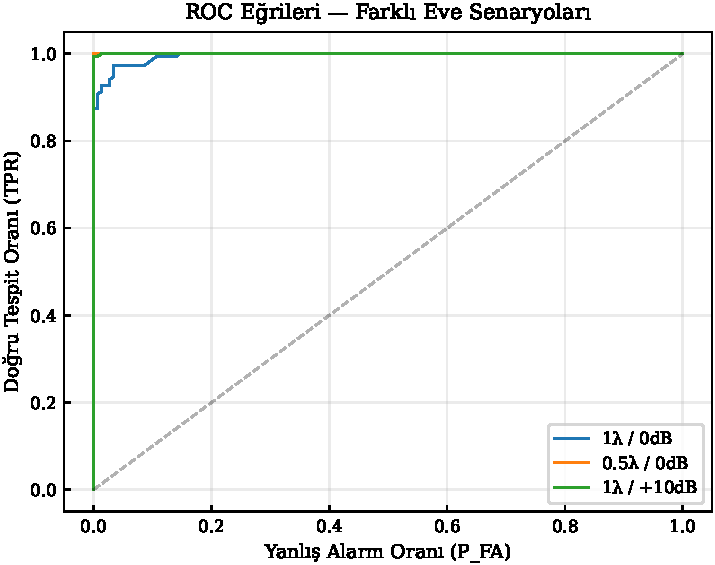
\includegraphics[width=\columnwidth]{figures/fig11_multi_roc.pdf}
\caption{Farklı Eve senaryolarında ROC eğrileri.}
\label{fig:multiroc}
\end{figure}

\begin{figure}[t]
\centering
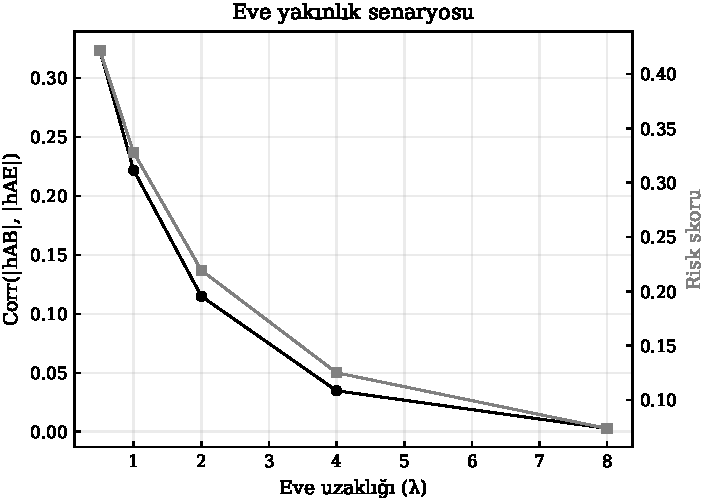
\includegraphics[width=\columnwidth]{figures/fig12_eve_distance.pdf}
\caption{Eve uzaklığının korelasyon ve risk skoruna etkisi.}
\label{fig:evedistance}
\end{figure}

Eve-Bob uzaklığı $\{0.5,1,2,4,8\}\lambda$ arasında taranmıştır (Şekil~\ref{fig:evedistance}). \SI{0.5}{\lambda} yakınlıkta ortalama risk skoru 0.40 ile orta seviyeye ulaşırken, \SI{4}{\lambda} ötesinde 0.14 altına düşmektedir. Tablo~\ref{tab:evesnr}'deki sonuçlar, Eve'in $\geq\SI{5}{dB}$ alıcı avantajında risk rejiminin düşükten ortaya geçtiğini göstermektedir.

\begin{table}[t]
\caption{Eve Alıcı Avantajı Senaryosu (\SI{1}{\lambda})}
\label{tab:evesnr}
\centering
\begin{tabular}{ccc}
\toprule
$\Delta SNR_E$ (dB) & Ort.\ risk & Sınıf \\
\midrule
$-10$ & 0.271 & Düşük \\
$-5$ & 0.295 & Düşük \\
0 & 0.320 & Düşük \\
5 & 0.385 & Orta \\
10 & 0.373 & Orta \\
\bottomrule
\end{tabular}
\end{table}

Elevasyon-yakınlık ısı haritası (Şekil~\ref{fig:heatmap}), düşük elevasyon (\SI{15}{\degree}) ve yakın Eve (\SI{0.5}{\lambda}) kombinasyonunun en riskli durum ($R_E=0.55$) olduğunu; yüksek elevasyon ve uzak Eve'de riskin 0.11'e düştüğünü ortaya koymaktadır.

\begin{figure}[t]
\centering
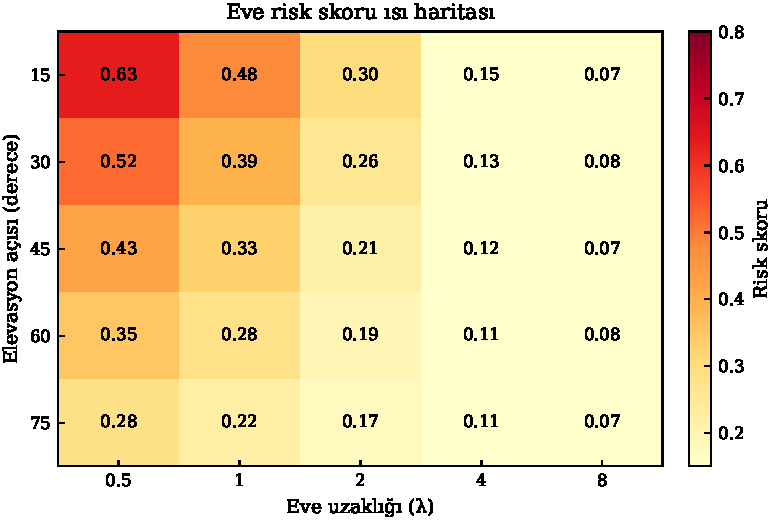
\includegraphics[width=\columnwidth]{figures/fig13_eve_heatmap.pdf}
\caption{Elevasyon-yakınlık risk skoru ısı haritası.}
\label{fig:heatmap}
\end{figure}

\subsection{Limitasyonlar}

Sonuçlar değerlendirilirken birkaç noktanın göz önünde bulundurulması gerekir. Birincisi, tüm analizler simülasyona dayanmaktadır; Loo model parametreleri ITU-R P.681'den alınmış olmakla birlikte gerçek uçuş verisiyle henüz doğrulanmamıştır. Kısmi doğrulama için DLR'nin yayımladığı L/S-band uydu kanal ölçüm veri setleri veya düşük maliyetli bir SDR (Software Defined Radio) platformuyla yer istasyonu deneyi uygun adaylar olup bir sonraki aşamada planlanmaktadır. İkincisi, Loo simülasyonunda Alice ile Bob arasında tam gölgeleme karşılıklılığı varsayılmıştır ki bu fiziksel olarak iyimser bir kabuldür ve saha testleriyle sınanmalıdır. Üçüncüsü, Eve'in uzaysal korelasyonu 0.15 olarak sabitlenmiştir; aynı yerel saçınıcı ortamın paylaşıldığı durumlarda (örneğin aynı bina içi) bu değer çok daha yüksek çıkabilir. Dördüncüsü, \SI{100}{Hz} örnekleme hızı senaryosunda $f_D \approx \SI{39}{kHz}$ Nyquist sınırını aştığından Doppler aliasing riski doğmaktadır; pratik bir sistemde kHz/MHz mertebesinde pilot hızlarına ihtiyaç duyulacaktır. Beşincisi, Eve yalnızca pasif dinleyici olarak modellenmiştir; pilot sinyal sahteciliği (pilot spoofing) veya ortadaki adam (man-in-the-middle) gibi aktif saldırı senaryoları kapsam dışıdır. Altıncı olarak, çalışma tek bir Alice-Bob çifti üzerine kuruludur; çok kullanıcılı veya mega-konstelasyon senaryolarında ölçeklenebilirlik ayrıca değerlendirilmelidir. Son olarak, NIST testleri tam bir teorik güvenlik garantisi değil, yalnızca istatistiksel bir sağlık göstergesidir.

%% ====================================================================
\section{Sonuç}
%% ====================================================================

Bu çalışmada, LEO uydu-zemin haberleşmesinde yayılım gecikmesi ile kanal tutarlılık süresi arasındaki uçurumu yavaş öznitelik çıkarımı ve AR kanal tahmini üzerinden ele alan bir hibrit güvenlik mimarisi ortaya konmuştur. Mimari; Cascade uzlaştırma, HMAC tabanlı anahtar evrimi ve ROC tabanlı Eve analizini tek bir protokolde toplamaktadır. Dinamik Loo geçiş benzetimlerinde \SI{20}{dB} SNR üzerinde ortalama \%1'in altında KDR, \SI{0.018}{bpcu} anahtar üretim hızı ve \%98'i aşan NIST geçme oranı elde edilmiştir. Öte yandan ideal karşılıklılık ve örnekleme hızı varsayımları nedeniyle bu sonuçların gerçek LEO donanımlarında tekrarlanması hâlâ gereklidir.

İleriye dönük olarak CRYSTALS-Kyber tabanlı kuantum sonrası anahtar kapsülleme entegrasyonu, derin öğrenme ile kanal tahmini, çok kullanıcılı ve mega-konstelasyon senaryolarına ölçekleme, aktif saldırgan modelleri (pilot spoofing, man-in-the-middle) ve gerçek uydu verisine dayalı doğrulama çalışmaları gündemdedir.

\section*{Teşekkür}
Bu çalışma herhangi bir dış fon desteği almaksızın, yazarların kişisel araştırma çabasıyla gerçekleştirilmiştir. Benzetim kodları ve üretilen veri setleri tekrarlanabilirlik amacıyla \url{https://github.com/onderozturk/leo-pkg-hybrid} adresinde açık kaynak olarak paylaşılmıştır.

%% ====================================================================
\begin{thebibliography}{30}

\bibitem{wyner}
A.~D. Wyner, ``The wire-tap channel,'' \emph{Bell Syst. Tech. J.}, vol.~54, no.~8, pp.~1355--1387, 1975.
\url{https://doi.org/10.1002/j.1538-7305.1975.tb02040.x}

\bibitem{maurer}
U.~M. Maurer, ``Secret key agreement by public discussion from common information,'' \emph{IEEE Trans. Inf. Theory}, vol.~39, no.~3, pp.~733--742, 1993.
\url{https://doi.org/10.1109/18.256484}

\bibitem{mathur}
S.~Mathur, W.~Trappe, N.~Mandayam, C.~Ye, and A.~Reznik, ``Radio-telepathy: extracting a secret key from an unauthenticated wireless channel,'' in \emph{Proc. ACM MobiCom}, 2008, pp.~128--139.
\url{https://doi.org/10.1145/1409944.1409960}

\bibitem{ye}
C.~Ye, A.~Reznik, Y.~Shah, W.~Trappe, and N.~Mandayam, ``Information-theoretically secret key generation for fading wireless channels,'' \emph{IEEE Trans. Inf. Forensics Security}, vol.~5, no.~2, pp.~240--254, 2010.
\url{https://doi.org/10.1109/tifs.2010.2043187}

\bibitem{bloch}
M.~Bloch and J.~Barros, \emph{Physical-Layer Security: From Information Theory to Security Engineering}.\ Cambridge, U.K.: Cambridge Univ. Press, 2011.
\url{https://doi.org/10.1017/cbo9780511977985}

\bibitem{cascade_orig}
G.~Brassard and L.~Salvail, ``Secret-key reconciliation by public discussion,'' in \emph{Proc. EUROCRYPT}, 1994, pp.~410--423.
\url{https://doi.org/10.1007/3-540-48285-7_35}

\bibitem{abdelsalam_state}
N.~Abdelsalam, S.~Al-Kuwari, and A.~Erbad, ``Physical layer security in satellite communication: State-of-the-art and open problems,'' \emph{IET Commun.}, vol.~19, no.~1, e12830, 2025.
\url{https://doi.org/10.1049/cmu2.12830}

\bibitem{bennett_lhl}
C.~H. Bennett, G.~Brassard, C.~Crepeau, and U.~M. Maurer, ``Generalized privacy amplification,'' \emph{IEEE Trans. Inf. Theory}, vol.~41, no.~6, pp.~1915--1923, 1995.
\url{https://doi.org/10.1109/18.476316}

\bibitem{chan_energy}
S.~Chan, S.~Kim, H.~W. Kim, B.-J. Ku, and D.-S. Oh, ``Energy-efficient physical layer security schemes for low Earth orbit satellite systems,'' \emph{Int. J. Satellite Commun. Netw.}, vol.~42, no.~5, pp.~374--396, 2024.
\url{https://doi.org/10.1002/sat.1519}

\bibitem{xiao_nextg}
Q.~Xiao, J.~Zhao, S.~Feng, G.~Li, and A.~Hu, ``Securing NextG networks with physical-layer key generation: A survey,'' \emph{Security and Safety}, vol.~3, Art.~2023021, 2024.
\url{https://doi.org/10.1051/sands/2023021}

\bibitem{torshizi}
E.~O. Torshizi and W.~Henkel, ``Pairwise physical layer secret key generation for FDD systems,'' \emph{IEEE Trans. Inf. Forensics Security}, vol.~19, pp.~9518--9533, 2024.
\url{https://doi.org/10.1109/TIFS.2024.3468170}

\bibitem{topal_doppler}
O.~A. Topal, G.~K. Kurt, and H.~Yanikomeroglu, ``Securing the inter-spacecraft links: Physical layer key generation from Doppler frequency shift,'' \emph{IEEE J. Radio Freq. Identif.}, vol.~5, no.~3, pp.~232--243, 2021.
\url{https://doi.org/10.1109/JRFID.2021.3077756}

\bibitem{liu_nextg}
Y.~Liu, H.-H. Chen, and L.~Wang, ``Physical layer security for next generation wireless networks: Theories, technologies, and challenges,'' \emph{IEEE Commun. Surv. Tutor.}, vol.~19, no.~1, pp.~347--376, 2017.
\url{https://doi.org/10.1109/COMST.2016.2598968}

\bibitem{yang_iot}
L.~Yang, Y.~Gao, J.~Zhang, S.~Camtepe, and D.~Jayalath, ``A channel perceiving attack and the countermeasure on long-range IoT physical layer key generation,'' \emph{Comput. Commun.}, vol.~191, pp.~108--118, 2022.
\url{https://doi.org/10.1016/j.comcom.2022.04.027}

\bibitem{3gpp}
3GPP, ``Study on security aspects of satellite access,'' 3GPP TR 33.700-28, V0.1.0, Release~18, Dec.\ 2023. [Çevrimiçi]. Erişim: \url{https://www.3gpp.org/dynareport/33700-28.htm} (Erişim tarihi: 15 Mar.\ 2025).

\bibitem{tua}
Türkiye Uzay Ajansı, ``Milli Uzay Programı,'' Strateji Belgesi, Ankara, Türkiye, Şubat 2021. [Çevrimiçi]. Erişim: \url{https://cdn.tua.gov.tr/60227c3d5f551.pdf} (Erişim tarihi: 15 Mar.\ 2025).

\bibitem{nist_pqc}
National Institute of Standards and Technology, ``Module-lattice-based key-encapsulation mechanism standard (FIPS 203),'' 2024.
\url{https://doi.org/10.6028/NIST.FIPS.203}

\bibitem{nist_sp800_22}
A.~Rukhin \emph{et al.}, ``A statistical test suite for random and pseudorandom number generators for cryptographic applications,'' NIST SP 800-22 Rev.~1a, 2010.
\url{https://doi.org/10.6028/NIST.SP.800-22r1a}

\bibitem{zhang_fdd_dnn}
X.~Zhang, G.~Li, J.~Zhang, A.~Hu, Z.~Hou, and B.~Xiao, ``Deep-learning-based physical-layer secret key generation for FDD systems,'' \emph{IEEE Internet Things J.}, vol.~9, no.~8, pp.~6081--6094, 2022.
\url{https://doi.org/10.1109/JIOT.2021.3109272}

\bibitem{zhang_fdd_ofdm}
X.~Zhang, G.~Li, J.~Zhang, L.~Peng, A.~Hu, and X.~Wang, ``Enabling deep learning-based physical-layer secret key generation for FDD-OFDM systems in multi-environments,'' \emph{IEEE Trans. Veh. Technol.}, vol.~73, no.~7, pp.~10135--10149, 2024.
\url{https://doi.org/10.1109/TVT.2024.3367362}

\bibitem{ldpc_recon}
M.~Bloch, A.~Thangaraj, S.~W. McLaughlin, and J.-M. Merolla, ``LDPC-based secret key agreement over the Gaussian wiretap channel,'' in \emph{Proc. IEEE ISIT}, 2006, pp.~1179--1183.
\url{https://doi.org/10.1109/isit.2006.261991}

\bibitem{polar_recon}
R.~A. Chou, M.~R. Bloch, and E.~Abbe, ``Polar coding for secret-key generation,'' \emph{IEEE Trans. Inf. Theory}, vol.~61, no.~11, pp.~6213--6237, 2015.
\url{https://doi.org/10.1109/tit.2015.2471179}

\bibitem{itur_p681}
ITU-R, ``Propagation data required for the design of systems in the land mobile-satellite service,'' Rec.\ P.681-11, Ağustos 2019. [Çevrimiçi]. Erişim: \url{https://www.itu.int/rec/R-REC-P.681-11-201908-I/en} (Erişim tarihi: 15 Mar.\ 2025).

\bibitem{itur_p618}
ITU-R, ``Propagation data and prediction methods required for the design of Earth-space telecommunication systems,'' Rec.\ P.618-13, Aralık 2017. [Çevrimiçi]. Erişim: \url{https://www.itu.int/rec/R-REC-P.618-13-201712-I/en} (Erişim tarihi: 15 Mar.\ 2025).

\bibitem{jorswieck}
E.~A. Jorswieck, S.~Tomasin, and A.~Sezgin, ``Broadcasting into the uncertainty: Authentication and confidentiality by physical-layer processing,'' \emph{Proc. IEEE}, vol.~103, no.~10, pp.~1702--1724, 2015.
\url{https://doi.org/10.1109/jproc.2015.2469602}

\bibitem{poor_schaefer}
H.~V. Poor and R.~F. Schaefer, ``Wireless physical layer security,'' \emph{Proc. Natl. Acad. Sci. USA}, vol.~114, no.~1, pp.~19--26, 2017.
\url{https://doi.org/10.1073/pnas.1618130114}

\bibitem{mukherjee}
A.~Mukherjee, S.~A. A. Fakoorian, J.~Huang, and A.~L. Swindlehurst, ``Principles of physical layer security in multiuser wireless networks,'' \emph{IEEE Commun. Surv. Tutor.}, vol.~16, no.~3, pp.~1550--1573, 2014.
\url{https://doi.org/10.1109/surv.2014.012314.00178}

\bibitem{ren_csi}
K.~Ren, H.~Su, and Q.~Wang, ``Secret key generation exploiting channel characteristics in wireless communications,'' \emph{IEEE Wireless Commun.}, vol.~18, no.~4, pp.~6--12, 2011.
\url{https://doi.org/10.1109/mwc.2011.5999759}

\bibitem{zeng_multipath}
K.~Zeng, D.~Wu, A.~Chan, and P.~Mohapatra, ``Exploiting multiple-antenna diversity for shared secret key generation in wireless networks,'' in \emph{Proc. IEEE INFOCOM}, 2010, pp.~1--9.
\url{https://doi.org/10.1109/infcom.2010.5462004}

\bibitem{lin_leo}
Z.~Lin, M.~Lin, B.~Champagne, W.-P. Zhu, and N.~Al-Dhahir, ``Secrecy-energy efficient hybrid beamforming for satellite-terrestrial integrated networks,'' \emph{IEEE Trans. Commun.}, vol.~69, no.~9, pp.~6345--6360, 2021.
\url{https://doi.org/10.1109/tcomm.2021.3088898}

\bibitem{loo_model}
C.~Loo, ``A statistical model for a land mobile satellite link,'' \emph{IEEE Trans. Veh. Technol.}, vol.~VT-34, no.~3, pp.~122--127, 1985.
\url{https://doi.org/10.1109/t-vt.1985.24048}

\bibitem{fontan_lms}
F.~P. Fontan, M.~Vazquez-Castro, C.~E. Cabado, J.~P. Garcia, and E.~Kubista, ``Statistical modeling of the LMS channel,'' \emph{IEEE Trans. Veh. Technol.}, vol.~50, no.~6, pp.~1549--1567, 2001.
\url{https://doi.org/10.1109/25.966585}

\bibitem{jana_eval}
S.~Jana, S.~N. Premnath, M.~Clark, S.~K. Kasera, N.~Patwari, and S.~V. Krishnamurthy, ``On the effectiveness of secret key extraction from wireless signal strength in real environments,'' in \emph{Proc. ACM MobiCom}, 2009, pp.~321--332.
\url{https://doi.org/10.1145/1614320.1614356}

\bibitem{oligeri_sat}
G.~Oligeri, S.~Sciancalepore, S.~Raponi, and R.~Di~Pietro, ``PAST-AI: Physical-layer authentication of satellite transmitters via deep learning,'' \emph{IEEE Trans. Inf. Forensics Security}, vol.~18, pp.~274--289, 2023.
\url{https://doi.org/10.1109/TIFS.2022.3219287}

\end{thebibliography}

\end{document}
